\chapter{Vývoj firmwaru}
V této kapitole se budem zabívat návrhem firmwaru s grafickým rozhraním pro mikrokontroler Raspberry pi 4, výběrem programovacího jazyku a ošetření nežádoucích stavů.

\section{Výběr programovacího jazyku}
Jako programovací jazyk jsem zvolil Python na základě jednoduché syntaxe a čitelnosti kódu. Python má rozsáhlé množství knihoven pro vývoj GUI aplikací a je také velmi populární v komunitě Raspberry Pi, což přináší spoustu dostupných zdrojů a podpory.

Další možností byly programovací jazyky C++ a C\#, které jsou výkonnější a vhodnější pro náročnější aplikace. Oproti Pythonu mají menší komunitní podporu a vývoj je pomalejší, což může byt velmi stěžejní pro vypracování této práce ve stanoveném termínu. C\# navíc není tolik platformě nezávislý jako Python a C++, proto pro některé aplikace, jako např. vývoj GUI není nejvhodnější.
%Zdroj: ChatGPT
%https://chat.openai.com/c/2b6bb45b-a5bb-4122-b076-c6c33868d2e9
%https://chat.openai.com/share/e9bd7c89-0ffb-462b-99e9-853263e092ca



\section{Vývoj grafického uživatelského rozhraní}

Grafické uživatelské rozhraní zkráceně GUI je prostředí díky kterému uživatel dokáže interagovat se zařízením prostřednictvím tlačítek, přepínačů, textových polí, ikon, zaškrtávacích políček a jiných grafických ovládacích prvků, které má vyobrazené na displeji zařízení.

\subsection{Výběr GUI frameworku}
Pro vývoj GUI jsem si vybral knihovnu s názvem Tkinter
.
.
.

\section{Hlavní okno}

Na hlavním okně budou zobrazeny veškeré informace o destilátu a naměřená data. Hlavní okno se objeví po načtení operačního systému a následném a mikrokontroleru

Při zapnutí mikrokontroleru a načtení operačního systému se firmware sám spustí a zobrazí se hlavní okno. Uživatel nemá možnost z tohoto okna "vyjet" do prostředí operačního systému. Zapnutí měřícího systému se provádí připojením napájecího kabelu, vypnutí následně přes vypínací tlačítko na displeji v sekci nastavení[č.x]
\\\\

\begin{figure}[!h]
    \begin{center}
        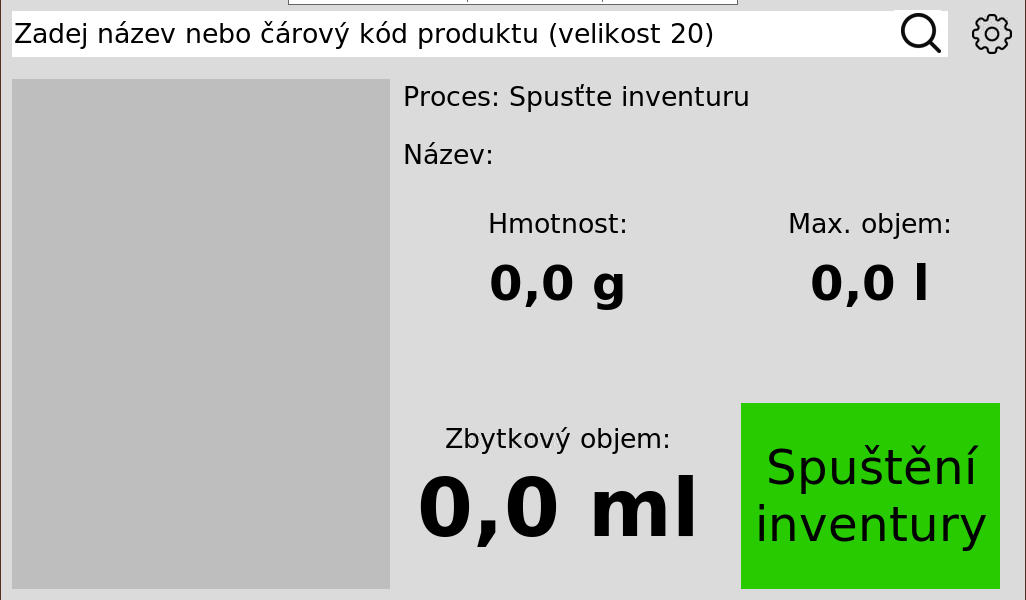
\includegraphics[scale=0.9]{obrazky/GUI.PNG}
    \end{center}
    \caption{GUI - Hlavní obrazovka}
    \label{putty}
\end{figure}

Komponenty hlavní obrazovky:
\begin{itemize}
    \item Tlačítko pro spuštění/ukončení inventury, zrušení výběru destilátu
    \item Tlačítko s ikonou ozubeného kolečka pro sekci nastavení
    \item Canvas pro zobrazení vybraného destilátu
    \item Entry(Text box) pro manuální vyhledávání destilátu
    \item 8x Label pro zobrazení hlavních informacích o měřeném destilátu
\end{itemize}

%\begin{minipage}{\linewidth}
%[frame=single,numbers=right,caption={Příklad %implementace první kanonické formy v~jazyce %C.},basicstyle=\ttfamily\small, %keywordstyle=\color{black}\bfseries\underbar,]

%Zde je možnost i barevného oddělení:
%https://www.overleaf.com/learn/latex/Code_listing
\begin{lstlisting}[language=Python, caption=Hlavní okno, frame=single]
import tkinter as tk
from PIL import ImageTk, Image

# Třída dědící z GUI knihovny Tkinter a třídy Tk
class Gui(tk.Tk):
    # Konstruktor
    def __init__(self):
        super().__init__()
        # Rozlišení hlavního okna
        self.geometry("1024x600")
        # Nastavení ostatních parametrů hlavního okna
                    .
                    .
                    .
    # Detekce zmáčknutí tlačítka
    def button_event_start_stop(self):
        self.button_start_stop_pressed = True

    # Otevře okno s nastavením
    def button_event_settings(self):
        exit()

    # Otevře okno dotykové klávesnice
    def entry_event(self, _event):
        keyboard = Keyboard(self)


\end{lstlisting}

///Zde bude obrazek hlavniho okna///

///Zde bude tabulka použitých komponent hlavního okna ///

///Zde bude kód/třída hlavního okna///

\subsection{Okno s nastavením}

Okno s nastavením se spouští pomocí ikony ozubeného kolečka.

///Zde bude obrázek okna s nastavením///

///Zde bude tabulka použitých komponent ///

///Zde bude kód/třída okna nastavení///

\subsection{Dotyková klávesnice}

Dotyková klávesa se otevře po kliknutí na textové pole s ikonou lupy. Slouží k vyhledání položky manuálně z důvodu poškozeného čárového kódu. Jednotlivé klávesy jsou tvořeny pomocí tk.button widgetu. Klávesnici je možné zavřít pomocí tlačítka close nebo kliknutím do prostoru mimo klávesnici.

\begin{figure}[!h]
    \begin{center}
        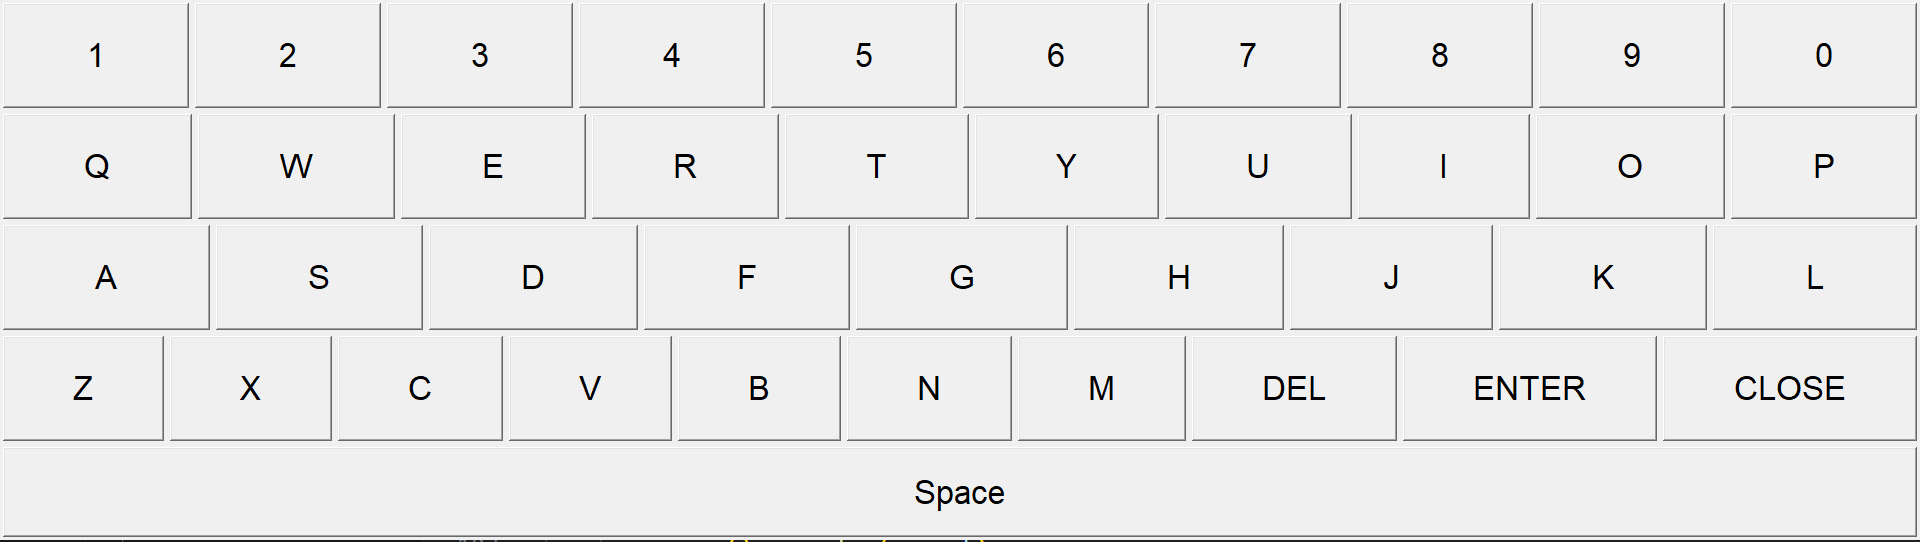
\includegraphics[scale=0.45]{obrazky/klavesnice.PNG}
    \end{center}
    \caption{GUI - Dotyková klávesnice}
    \label{putty}
\end{figure}

\begin{lstlisting}[language=Python, caption=Hlavní okno, frame=single]
class Keyboard(tk.Toplevel):,
    def __init__(self, parent):
        super().__init__(parent)
        self.parent = parent
        self.geometry("1024x300+0+300")  # Nastavení rozměrů a pozice okna na spodní polovinu obrazovky
        self.overrideredirect(True)  # Odstraní vrchní lištu s tlačítky minimalizace, maximalizace a zavření

        # Inicializace klávesnice
        self.init_keyboard()

    def init_keyboard(self):
        # Funkce pro zachycení stisku klávesy
        def press(key):
            if key == "ENTER":
                pass  # Potvrzení vyhledávání nebo tu může být zavření klávesnice...uvidím
            elif key == "DEL":
                current_text = self.parent.entry.get()
                new_text = current_text[:-1]  # Odstranění posledního znaku
                self.parent.entry.delete(0, tk.END)  # Vymazání současného textu
                self.parent.entry.insert(0, new_text)  # Vložení upraveného textu
            elif key == "Space":
                self.parent.entry.insert(tk.END, " ")
            elif key == "CLOSE":
                self.wm_withdraw()
            else:
                self.parent.entry.insert(tk.END, key)

        # Definování velikosti písma pro klávesy
        font_size = "20"

        # Vytvoření rámce pro klávesy
        frame = tk.Frame(self)
        frame.pack(expand=True, fill='both')

        # Layout kláves s přidanou numerickou řadou
        keys = [
            ['1', '2', '3', '4', '5', '6', '7', 
            '8', '9', '0'],
            ['Q', 'W', 'E', 'R', 'T', 'Y', 'U', 
            'I', 'O', 'P'],
            ['A', 'S', 'D', 'F', 'G', 'H', 'J', 
            'K', 'L'],
            ['Z', 'X', 'C', 'V', 'B', 'N', 'M', 
            'DEL', 'ENTER', 'CLOSE'],
            ['Space']
        ]

        # Vytvoření kláves
        for row in keys:
            row_frame = tk.Frame(frame)
            row_frame.pack(
                side='top', 
                expand=True, 
                fill='both')
            for key in row:
                if key == "Space":
                    button = tk.Button(
                    row_frame, 
                    text=key, 
                    command=lambda k=key: press(k), 
                    height=2, 
                    font=("Helvetica", font_size), 
                    width=87)
                    button.pack(
                    side='left', 
                    expand=True, 
                    fill='both', 
                    padx=3, 
                    pady=3)
                else:
                    button = tk.Button(
                    row_frame, 
                    text=key, 
                    command=lambda k=key: press(k), 
                    height=2, 
                    font=("Helvetica", font_size), 
                    width=7)
                    button.pack(
                    side='left', 
                    expand=True, 
                    fill='both', 
                    padx=3, 
                    pady=3)


\end{lstlisting}

\section{Hlavní soubor} %\section{Stavový automat}

%Hlavní soubor "main.py" se spouští jako první a následně na základě stavového automatu volá ostatní

Hlavní soubor "main.py" je spouštěcí soubor, kde sekvence úkolů je závislá na stavovém automatu. Stavy stavového automatu jsou tvořeny enum třídou ve kterém je definován každý stav. Rozhodovácí část stavového automatu je ve funcki "state\_machine", která je volána z mainu s počátečním stavem pro spuštění inventury, na základě stavu jsou volané dílčí funkce určene pro každý stav. Tato funkce je dokola volána díky metody tkinter.after() z důvodu, že program běží na hlavní smyčce grafické třídy Tkinter a intervalu 100 je volána opakovaně funkce state\_machine.

\begin{figure}[!h]
    \begin{center}
        \includegraphics[scale=0.45]{obrazky/stavový automat_2.jpg}
    \end{center}
    \caption{Stavový automat programu}
    \label{putty}
\end{figure}

\begin{lstlisting}[language=Python, caption=Hlavní okno, frame=single]
from enum import Enum

class automat(Enum):
    spusteni_inventury = 1
    finding_the_distillate = 5
    stav2 = 2
    stav3 = 3
    stav4 = 4
\end{lstlisting}

\newpage

\begin{lstlisting}[language=Python, caption=Hlavní okno, frame=single]
def state_machine(state: automat) -> None:
    
    #switch statement by "if" condition (Python version 3.9.2)
    if state == automat.spusteni_inventury and
    app.button_start_stop_pressed:
        state = starting_inventory()
    elif state == automat.finding_distillate:
        state = finding_distillate()
    elif state == automat.weighing():
        state = weighing()
    elif state == automat.remove_() and 
    vaha.print_scale().split()[0] == "0.0":
        state = remove_bottle()

    if state != automat.spusteni_inventury and 
    state != automat.stav3 and 
    app.button_start_stop_pressed:
        stop_inventory()
        state = automat.spusteni_inventury

    app.after(100, state_machine, state)
\end{lstlisting}

\subsection{Stav: Zahájení inventury}
Zahájení inventury probíhá pomocí sepnutí tlačítka pro spuštění inventury. Tento stav kontroluje zda komunikační port váhy a čtečky čárového kódu je otevřený a vytváří novou tabulku v databázi pro ukládání dat navážených destilátů.

\begin{lstlisting}
    def starting_inventory() -> automat:
\end{lstlisting}

\newpage
\subsection{Stav: Hledání destilátu}

V tomto stavu se posílá opakovaně požadavek na skenování pomocí skeneru čárového kódu, dokud se ho nepovede přečíst. Získaný EAN kód se porovná s ostatními v databázi, při neshodě se vypíše chybové hlášení, že EAN kód se nenašel. Při shodě se zjistí, zda nebyl už evidován destilát s tímto EAN kódem z důvodu vyhnutí se duplicitní evidenci. Při shodě se vypíše chybové hlášení, že položka už byla evidována. Pokud byl EAN kód uspěšně načten, aktualizují se informace na dipsleji pro načtený destilát.

\begin{lstlisting}
    def finding_distillate() -> automat:
\end{lstlisting}

\subsection{Stav: Vážení}

%Zrušení výběru je možné pomocí tlačítka
Pokud naměřená hmotnost je větší než hmotnost plné láhve, vypíše se "MAX" místo hodnoty zbytkového objemu. Jedná se o ošetření chyby pokud by na váhu byla položena špatná láhev nebo jiný objekt s větší hmotností, než je hmotnost plné lahve. Pokud váha je stabilizovaná, posílá po sériové lince naměřenou hmotnost včetně jednotky[tab. č.\ref{jouu}], pokud tedy je přijata jednotka hmotnosti a hmotnost je současně vyšší než hmotnost prázdné láhve, tak se podbarví zeleně jednotka zbytkového objemu, jako signalizace stabilizované váhy a destilát se nám eviduje do databáze.

\begin{lstlisting}
    def weighing() -> automat:
\end{lstlisting}

\subsection{Stav: Odebrání láhve}

Pokud naměříme nulovou hmotnost na váze, tak se nám vynuluje zbytkový objem a systém se dostane do stavu pro hledání

\begin{lstlisting}
    def remove_bottle() -> automat:
\end{lstlisting}

\subsection{Stav: Ukončení inventury}

Tento stav nastane, když je aktivováno tlačítko pro ukončení inventury a zároveň nejsme ve stavu vážení ani spuštění inventury. Po dokončení inventury je možné zahájit další inventuru. Pokud uživatel zamýšlí zahájit novou inventuru bez restartování zařízení, systém se ho zeptá, zda si přeje smazat předchozí inventuru(viz obrázek č.). Důvodem pro zahájení nové inventury může být chyba v předchozí inventuře.

\begin{lstlisting}
    def stop_inventory() -> automat:
\end{lstlisting}

\begin{figure}[!h]
    \begin{center}
        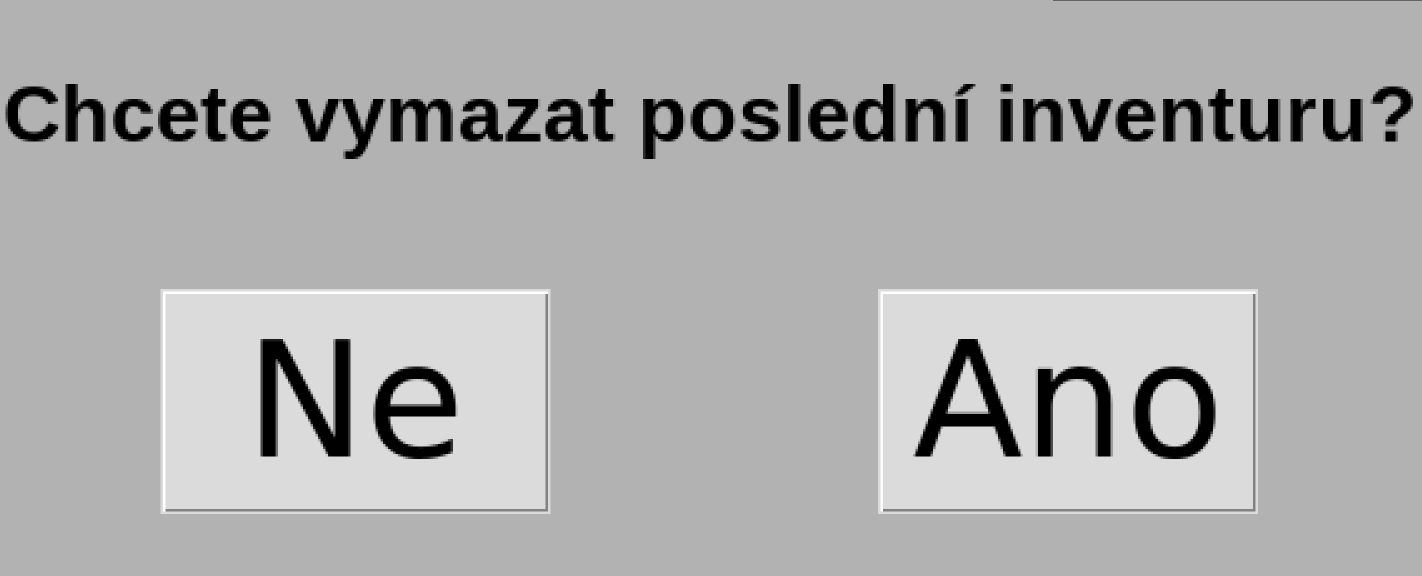
\includegraphics[scale=0.45]{obrazky/mazani_inventury.PNG}
    \end{center}
    \caption{Systémové okno pro vymazání poslední inventury}
    \label{putty}
\end{figure}

\section{Třída váhy}

Třída váhy "scale" zastřešuje sériovou komunikaci s váhou. 

V konstruktoru je vytvořena instance třídy pro sériovou komunikaci s parametrim timeou=1, který nastavuje, čtená na seriovém portu po dobu 1 s. Pokud do tohoto intervalu nejsou zaznamenány žádné příchozí data, čtení se ukončí. 

Metoda "open\_port" otevírá port pro komunikaci, pokud už port nebyl otevřen nebo neselže jeho otevření. Výjimka "serial.SerilException" se vyvolá pokud na portu není fyzicky připojený kabel. Návratovou hodnotou je bool zda se povedlo otevřít port.

Metoda "print\_scale" posílá váze požadavek pro zpětné odeslání navážené hmotnosti. Váha přijíma a odesíla data v ASCII formátu. Pokud do 1s nepřijmeme data, funkce vrátí "Err0". Tato funkce stále kontroluje zda je port otevřený, v případě uzavřeného portu vrací hodnotu "Err1". Při úspěšném přečtení dat na portu vrátí funkce přečtená data

Metoda is\_open" kontroluje zda je port otevřený pomocí proměnné "is\_open" třídy "serial". Návratová hodnota je bool na základě zda port je otevřený nebo ne.

-------------------------

Třída Scale zastřešuje sériovou komunikaci s váhou.

V konstruktoru se vytváří instance třídy serial.Serial pro sériovou komunikaci s parametrem timeout=1, který nastavuje, že čtení na sériovém portu bude probíhat po dobu 1 sekundy. Pokud během této doby nejsou zaznamenána žádná příchozí data, čtení se ukončí.

Metoda open\_port otevírá port pro komunikaci, pokud již není otevřen, a pokud jeho otevření neproběhne úspěšně. Výjimka serial.SerialException je vyvolána, pokud na portu není fyzicky připojený kabel. Návratovou hodnotou je bool, který indikuje, zda se podařilo port otevřít.

Metoda print\_scale posílá váze požadavek pro zpětné odeslání navážené hmotnosti. Váha přijímá a odesílá data v ASCII formátu. Pokud do 1 sekundy nepřijmeme data, funkce vrátí "Err0". Tato funkce také kontroluje, zda je port otevřený, a v případě uzavřeného portu vrací hodnotu "Err1". Při úspěšném přečtení dat na portu vrátí funkce přečtená data.

Metoda is\_open kontroluje, zda je port otevřený pomocí proměnné is\_open třídy serial. Návratová hodnota je bool na základě toho, zda je port otevřený nebo ne.

\begin{figure}[!h]
    \begin{center}
        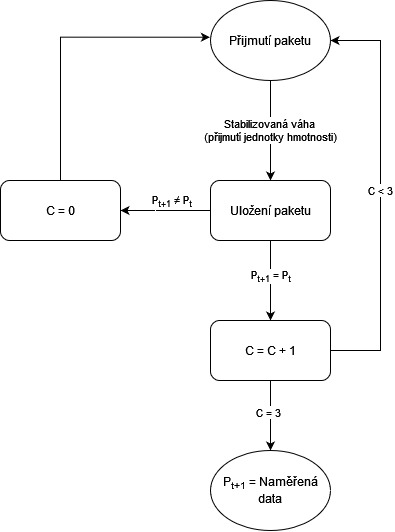
\includegraphics[scale=0.8]{obrazky/stavovy_automat_parita.jpg}
    \end{center}
    \caption{Systémové okno pro vymazání poslední inventury}
    \label{putty}
\end{figure}

\begin{lstlisting}[language=Python, caption=Hlavní okno, frame=single]
import serial

class scale:

    def __init__(self) -> None:
        self.vaha = serial.Serial(timeout=1)

    def open_port(self) -> bool:
        if not self.vaha.is_open:    
            try:
                self.vaha.port = '/dev/ttyUSB0'
                self.vaha.open()
            except serial.SerialException:
                return False
        return True

    def print_scale(self) -> str:
        try:
            data = chr(27).encode('utf-8')
            +chr(112).encode('utf-8')
            self.vaha.write(data)
            self.catch_data = self.vaha.readline().decode()
            if self.catch_data == '':
                return "Err0"
        except serial.SerialException:
            if not self.open_port():
                return "Err1"
        return self.catch_data
    
    def is_open(self) -> bool:
        if self.vaha.is_open:
            return True
        else:
            return False
\end{lstlisting}

\section{Třída čtečky čárového kódu}

%Ve funkci print\_sensor třídy sensor pošlem senzoru zprávu xxx
Metoda print\_sensor funguje na základě trigger modu čtečky čárového kódu viz kapitola č. \ref{zprovozeni_ctecky}. Senzoru pošlem zprávu xxx, po jeho přijetí senzor pošle zpět zprávu "31" v ASCII a začne skenovat po dobu xxx s. Ve while smyčce kontrolujeme zda došel poslední znak "1". Následně začnem do bufferu načítat data, dokud nenarazíme na koncový znak "\r". Návratová hodnota je str obsahující data z bufferu.

\begin{lstlisting}[language=Python, caption=Ukázka třídy pro čtečku čárového kódu, frame=single]
import serial
import time

class sensor:

    def __init__(self) -> None:
        self.senzor = None
        self.scan_duration = 5
        try:
            self.senzor = serial.Serial(
            '/dev/ttyACM0', 
            9600, 
            timeout=0)
        except serial.SerialException:
            print("Port se nepovedl otevřít - ČTEČKA")
    
    #Senzor s trigger modem
    def print_sensor(self):
        
        scan_command = b'\x7E\x00\x08\x01\x00\x02\x01\xAB\xCD' #Požadavek pro čtení    
        self.senzor.write(scan_command)
        time.sleep(0.1)

        while True:
           if self.senzor.read().decode() == '1' 
           or self.senzor.read().decode() == ''
                break

        start_time = time.time()
        data = ''

        while (time.time() - start_time) <= self.scan_duration:
            byte = self.senzor.read().decode()
            if byte == '\r':
                break
            else:
                data += byte

        return data
\end{lstlisting}

\section{Modul pro práci s databází}

Pro vytvoření databáze jsem si zvolil 

\begin{lstlisting}[language=Python, caption=Ukázka třídy pro čtečku čárového kódu, frame=single]
from sqlalchemy import Column, Integer, Numeric, String, create_engine, Table, MetaData, insert
from sqlalchemy.ext.declarative import declarative_base
from sqlalchemy.orm import sessionmaker
from datetime import datetime
import logging

Base = declarative_base()
last_table:str = None
logging.basicConfig(level=logging.INFO, format='%(asctime)s - %(levelname)s - %(message)s')

class Destilaty(Base):
    __tablename__ = 'destilaty'
    
    name = Column(String, primary_key=True)
    ean = Column(Integer)
    max_volume = Column(Numeric)
    weight_empty = Column(Numeric)
    weight_full = Column(Numeric)
    image = Column(String)

class Nalevac(Base):
    __tablename__ = 'nalevac'
    
    name = Column(String, primary_key=True)
    manufacturer = Column(String)
    weight = Column(Numeric)
    image = Column(String)
     
class Inventory(Base):
    __tablename__ = 'inventory'

    name = Column(String, primary_key=True)
    volume = Column(Integer)
    #popripade pridani info o času a datu měření


# Create an engine that stores data in the local directory's
# sqlalchemy_example.db file.
engine = create_engine('sqlite:///bakalarka.db')
engine_inventory = create_engine('sqlite:///inventory.db')

Base.metadata.create_all(engine_inventory, tables=[Inventory.__table__]) #Pokud už databáze a její tabulky existují, nemusíme volat tuto metodu 

# create a configured "Session" class
Session = sessionmaker(bind=engine)
Session_inventory = sessionmaker(bind=engine_inventory)

# create a Session
session = Session()
session_inventory = Session_inventory()

def create_new_inventory_table() -> None:
    try:
        # Získání aktuálního data a času
        current_time = datetime.now()
        table_name = current_time.strftime("inventory_%Y_%m_%d_%H%M%S")

        # Dynamické vytvoření nové třídy tabulky
        attrs = {
            '__tablename__': table_name,
            #'id': Column(Integer, primary_key=True),
            'name': Column(String, primary_key=True),
            'volume': Column(Integer),
            '__table_args__': {'extend_existing': True}
        }
        
        # Dynamické vytvoření nové třídy pomocí type
        NewTable = type(table_name, (Base,), attrs)
        
        # Vytvoření tabulky v databázi
        Base.metadata.create_all(engine_inventory, tables=[NewTable.__table__])

        global last_table
        last_table = table_name
        logging.info(f"Tabulka '{table_name}' byla úspěšně vytvořena.")
    except Exception as e:
        logging.error(f"Nastala chyba při vytváření tabulky: {e}")

def get_info(ean: str) -> list[Destilaty]:
    session = Session()
    results = session.query(Destilaty).filter(Destilaty.ean == int(ean)).all()
    session.close() #uzavření session, aby nedoslo k poškození dat nahodou
    return results

def find_data(aName: str) -> bool:
    session = Session_inventory()
    existing_entry = session.query(Inventory).filter_by(name=aName).first() #kontrola zda nepřídávám už existující prvek
    session.close()
    return existing_entry

def write_data(aName, aVolume) -> None:
    if last_table is None:
        logging.error("Nebyla vytvořena žádná tabulka pro zápis dat.")
        return
    
    try:
        # Připojení k existující tabulce
        metadata = MetaData()
        metadata.reflect(bind=engine_inventory)
        existing_table = metadata.tables[last_table]
        
        # Vložení dat do tabulky
        stmt = insert(existing_table).values(name=aName, volume=aVolume)
        with engine_inventory.connect() as connection:
            connection.execute(stmt)
            connection.commit()
        
        logging.info(f"Data byla úspěšně zapsána do tabulky '{last_table}'.")
    except Exception as e:
        logging.error(f"Nastala chyba při zápisu dat do tabulky '{last_table}': {e}")

\end{lstlisting}

\section{Nastavovací okno}
Nastavovací okno se otvírá kliknutím na ozubené kolečko hlavního okna. Okno obsahuje nastavení jednotek jednotlivých měřených veličin viz obr. č.() a tlačítko pro vypnutí mikrokontroleru. Kod je definován třídou Settings\_window v modulu GUI.

%Kod se nachátí v GUI modulu pod třídou 

\begin{figure}[!h]
    \begin{center}
        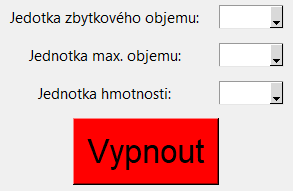
\includegraphics[scale=2]{obrazky/settings_okno.PNG}
    \end{center}
    \caption{Nastavovací okno v defaultním stavu}
    \label{putty}
\end{figure}


///Zde bude obrázek okna klávesnice///

///Zde bude tabulka použitých komponent ///

///Zde bude kód/třída okna klávesnice///

jebebebebebebeadjhasdjasjdasd

haha

hiohi